\chapter{Design}
This chapter will focus on the prototype VR application which will be implemented. Before starting with the development, the content of the  application has to be set. Also the requirements of the application have to be clear. For which target group the application is developed? What is the storyline of the application? How will the application be used later on? In the following, it will be shortly introduced, how the mode of operation is done during the implementation. After that the requirements will be set. A target user group for the VR application will be set, in order to start with the storyline. The application will have a fictive storyline, similar to a computer game. In order to design the story, a storyboard was created and will be presented in this chapter. Once the content is set, the thesis will take a look at HMDs and choose the suitable hardware device for the implementation.
\section{Mode of operation}
The objective of this thesis is to develop and evaluate a prototype VR application to display the different IT courses offered at NYP. To handle a complex task like this, it is important to apply a suitable mode of operation. For the design and development part of this thesis an agile approach is chosen. This means that the planning is done in an iterative process to remain flexible towards unexpected challenges. An agile approach does not mean that the main objective will change, but the task planning is adapted for one period and can be changed and evaluated after each iteration. Specifically for this thesis, there are weekly updates with the supervisor. During meetings, the work is reviewed and evaluated. Every six week there is a presentation of the work done for the last period and the tasks for the next six weeks are planned.\\
Each IT course, which is planned to be represented in the VR application will be treated separately. This means, that during an iteration, not more than one job role will be in focus of the design and development part.  

\section{Requirements}
The application focuses on prospective students as users. After using the VR application, they should have a clearer understanding, what the IT courses offered at NYP are about. Also they should gain a basic understanding about the jobs they can attend after getting a diploma in IT. In order to achieve this, several functional requirements have to be set:\\
\begin{itemize}
\item Introduction of IT job roles: The application should introduce to the user, what the job roles are about.
\item Start scene: The application starts in a futuristic city which can be explored by the user.
\item Interaction with items: The user can interact with several objects in the starting scene and enter different scenes through this.
\item Separation of each job role: Each job role should be presented in a separate scene. The user should be aware of which job role the scene is referred to at all times.
\item Completing tasks: Each introduction of a job role should contain information of the job and a task which should be completed by the user.
\item Following a main story line: There should be a main objective and each job role task is a step towards completing the main objective.
\item Gamification: The tasks should be structured as minigames and there should be a reward after completing them successfully.

\end{itemize}
Besides the functional requirements, there are several non-functional requirements which have to be considered when developing the prototype:
\begin{itemize}
\item Setting: The application should take place in a futuristic environment. Users should see how they can impact the future with IT.
\item Genre: The application should be a mix between a informative educational and a gaming application.
\item Educational: The user should gain more knowledge of the IT job roles after playing the VR application.
\item Portable: The application should be presented at various public events, such as open houses or fairs.
\item Budget: The product will not be distributed commercially. Therefore the costs for external tools, graphic or audio assets should be held to a minimum.
\end{itemize}

\section{Stakeholders}
This chapter defines the different actors for the VR application. After answering the question of what to do, we will answer the question of who will do it. This will be done by naming the different stakeholders of the application.
\begin{itemize}
\item School of Information Technology
\item Project leader
\item Prospective students
\item Developer
\end{itemize}
These stakeholders have different interests and expectations to the project. The School of Information Technology would like to have more students signing up for an IT course. They expect that the VR application arouses interest in IT by prospective students. Their task is to provide the application at public events, such as open houses and similar events. The School of Information Technology is also responsible for providing the IT courses which are introduced in the VR application. \\
The project leader expects a structured and well communicated application development. They expect that the objectives of the work is clear and the deadlines are met. The project leader is responsible for the guidance of the developers and the communication between the customer (School of IT) and the developers. The project leader sets and monitors the milestones in collaboration with the developers.\\
The prospective students are the end users of the VR application. They expect a diverting experience while using the application. They also want to learn more about the IT courses offered at NYP. Their task is to play the actual application. In case they are interested in one of the IT courses, they are responsible in applying for a diploma course at NYP.\\
The developers expect clear objectives from the project leader and a detailed description of the requirements. Their responsibility is to provide the actual application based on the frame given by the project leader and the customer. They develop a storyline, program the application and test it as well. In close communication with the project leader, they apply changes to the system.
\section{Target group}
\todo{outlining target group: prospective students; creating persona}
Before starting with the design of the application, a target group has to be defined. This makes developing of the application purpose easier and also helps not to loose the focus during the design process. A very important aspect of defining a target group is also, to develop the application directly to the needs of the future users. In the end this helps to increase the acceptance of the application. 

The main target group of the virtual reality application will be prospective students, who are thinking of taking a diploma at NYP. As mentioned in the introduction, those students mostly come from a secondary school and have finished their O-Levels, which is an entry requirement for polytechnics. The secondary school educated the students on a very widespread basis, and the students can now decide their specialisation. \\
When the students leave their secondary school, the average age is 16. In this age, people are known to be open to new technologies and trends. Also, the people in the target group are in the stage to make independent decisions for themselves without influence of parents. The application will be designed for prospective student, which show an interest in information technology but yet have no experience or knowledge in that field.\\
In the following, a characteristic of a fictive person is displayed. This person stands as a representative for the target group of prospective students:

\paragraph{Characteristics}
\begin{description}
	\item[Name:] Jessica Lee
	\item[Age:] 16
	\item[Place of residence:] Singapore
	\item[Education:] Finished secondary school
	\item[Personal interests:] Dancing, computer games, TV series, technology
	\item[Level of tech experience:] Rich consumer, no programming skills
	\item[Expectation:] Wants to experience a fun virtual reality application
\end{description}
Since the fictive person Jessica Lee's main expectation is to experience a joyful application, there will be the need of gamification elements in the application. Her interests in computer games and technology lead the application's scene setting into a futuristic environment with new technologies. She has experience in digital media as a consumer, but not as a professional (programmer). Therefore, common gestures for user interaction can be applied, but the difficulty level of tasks about information technology should be on a beginner level. 
\section{Main story concept}
To gain the users attention and let them grow interest in the application it is important to have a good main story. The main story will create a bridge between the several IT courses displayed in the application.\\
The application will start in the so called ``Smart City''. This is a futuristic urban environment in which the user can move around freely.There are five different buildings along the streets. Each building is interactive and represents a course offered by the NYP. By interacting with the buildings the user can enter laboratories, so called ``labs'', and complete different tasks. Every successful completion of a task has an impact to the main story. \\
The main goal of the VR application is to create a delivery drone which will deliver orders from online shops, just like Amazon announced in a video of 2013 (source). This is still a vision of future for now, but it is a good showcase for the user to show them how they can impact the future with IT. During the completion of the labs several challenges will occur. Once the user started programming their first drone, a lot more drones will start flying around in Smart City. To avoid crashing and chaos, the next task is to provide a proper and stable internet connection to the drones, so they can communicate. But the connected drones have their advantages and disadvantages: At first they are flying normally and communicating to each other but then an unknown IoT-Hacker infiltrates a virus into the drone firmware, so they start to misbehave. Now the user has to trace the hacker with basic cyber security concepts. After the hacker was found, more and more inhabitants of Smart City start to use the drones and provide a lot of data. It is now the job of the user to analyse this data and optimise the drones. By combining relevant data, it is possible to add some enhancements to the drone.
Once the user completed all tasks and visited all labs, the user can exit the game. \\
It has to be mentioned that not all courses offered by NYP are covered in this main story so far. This is the case, because the application prototype will concentrate on the job role of the software engineer and the cyber security analyst. Other job professions will be added in an iterative process.

\section{Storyboard}
In this chapter, the structure and the details of the main storyline are explained with the use of a storyboard. Since the requirements for the prototype application are already set, the storyboard points out the details of the requirements in a visual way.
The main objective of a storyboard is to get a scene by scene overview of the story and the sequence of events. Through a sketch draft, an idea of the visuals of the application is displayed. Still the focus of the storyboard lies on the storyline. Logical orders of scenes are displayed through arrows, textual explanations are added, whenever necessary.\\
For the storyboard of the prototype, a tool called invision freehand is used \cite{TODO}. In the following, some important parts of the storyboard are presented. The complete storyboard can be seen in \cite{TODO}.
\subsection{World scene and software engineer scene}
\begin{figure}[h!]
  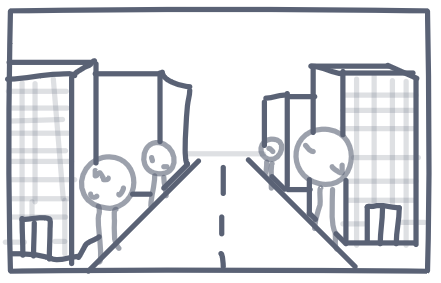
\includegraphics[width=8cm]{kapitel/storyboard/smart-city.PNG}
  \centering
  \caption{Smart city scene from where the user can explore different IT job roles.}
  \label{fig:smartcity}
\end{figure}
The first scene of the storyboard is the smart city scene, as sketched in figure \ref{fig:smartcity}. Here the user can walk around freely. When clicked on the software engineer building, an assistant asks the user to enter the building. If answered with "yes", there is a transition into the software engineer laboratory scene. The laboratory contains a testing drone and a package as well as working desks with laptops. After the transition, the assistant explains the first task, as displayed in \ref{fig:sescene}. This is the first minigame, in which the user should gain understanding in how programming works.
\begin{figure}[h!]
  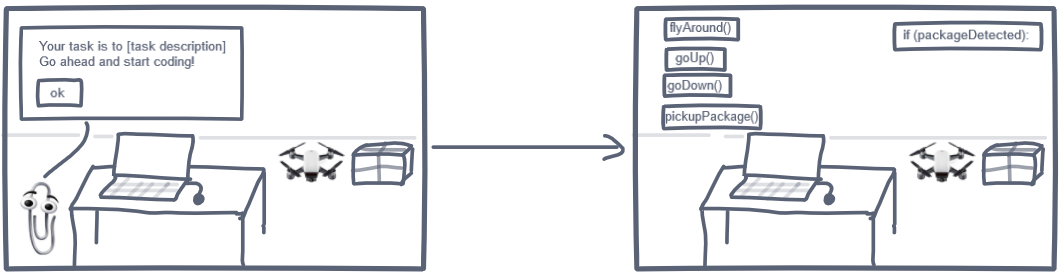
\includegraphics[width=16cm]{kapitel/storyboard/se-scene.PNG}
  \centering
  \caption{Software engineer scene: dialog and minigame}
  \label{fig:sescene}
\end{figure}
\\The information is taught in a very simplfied way, because the requirements of the application are, that it is playable without knowledge in IT. The objective of the task is to program the package delivery drone, so that it actually picks up a package. This is done by arranging lines of code in a logical order. The working environment is a desk with a laptop. After the user has arranged and ran the code successfully, they can watch the testing drone in the lab picking up the package. With the completion of this minigame, the scene ends and the user is transferred back to the world scene.
\subsection{Cyber security specialist scene}
The second scene represents the job role of the cyber security specialist. The scene is a laboratory with several office working places and the drone from the previous scene, which is displayed on a table in the middle of the room. When the user enteres the lab, it is explained, that the drone, they had programmed before, was corrupted by an unknown hacker. During the next task, the user should gain knowledge in the methods, cyber security specialists use to investigate digital crimes. The user learns about simple data decoding and encoding as well. The minigame is divided into three parts. 
\begin{figure}[h!]
  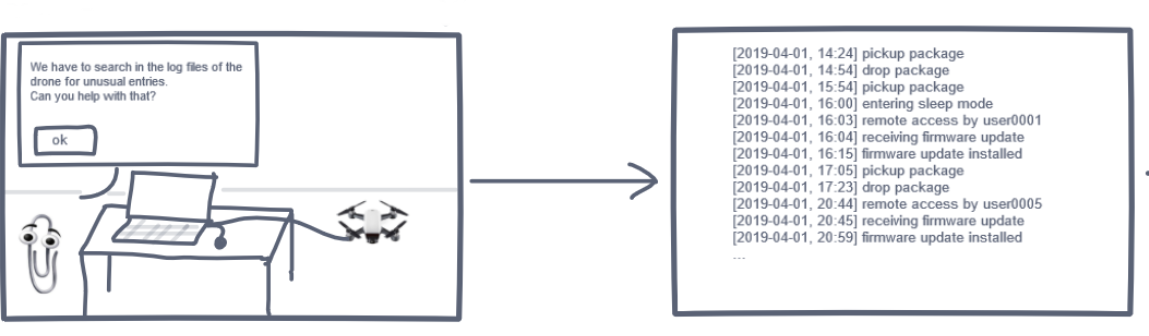
\includegraphics[width=16cm]{kapitel/storyboard/cyber-analyst1.PNG}
  \centering
  \caption{Cyber security specialist scene: searching log entries}
  \label{fig:logscene}
\end{figure}
\\In the first part, the user searches the log data of the drone for unauthorized access and marks suspicious entries, which can be seen in figure \ref{fig:logscene}. It turned out that two lab employees have accessed the drone during the last 24 hours. The second part of the minigame is to search the computers of the two lab employees for further information. 
\begin{figure}[h!]
  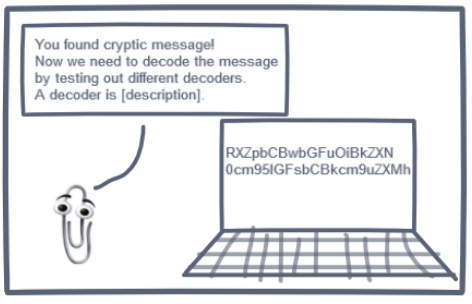
\includegraphics[width=8cm]{kapitel/storyboard/cyber-analyst3.PNG}
  \centering
  \caption{Cyber security specialist scene: encrypted message}
  \label{fig:logscene2}
\end{figure}
One employee has an encoded message on their desktop (figure \ref{fig:logscene2}).\\ The last part is to decode the message by trying out different commonly used codes. The message reveals the hacker and the person can be prosecuted. This marks the end of the cyber security specialist scene.

%\section{Hardware evaluation}
%Looking at the requirements, one of the constraints for the application is, that it should be portable. Another requirement is, that the budget should be held to a minimum. This limits the number of hardware devices, which can be used within the VR application. When it comes to choosing a HMD, there is the decision between mobile HMD and desktop HMD. Since a mobile HMD fulfills the requirement of portability better than the dektop linked version, this is the preferred HMD.\\
\newpage
\section{Dialogue design}
As seen in the storyboard, the application will contain a lot of conversation between the assistant and the user. Therefore, a decision has to be made on how to realise conversations in VR. The dialogues are indeed very important for the game, because most of the relevant information about the IT professions are given through the conversation with the user. The dialogues should be presented in a natural and interesting way, because the application should arouse interest in IT job roles and the user should not perceive the conversations as lengthy.\\
In the previous chapter different ways of designing a dialogue system were already mentioned. This section will now determine and evaluate the most useful dialogue system based on the above mentioned objective. Also the decision has to be made under the aspect of simplicity, time and budget.\\
Spoken dialogue systems may be the most natural way of communication, but on the other hand are not easy to realise and need a lot of computation. This application will therefore stick with a text based dialogue system. To still provide a natural experience to the user, the dialogues should be mixed with interactions. Nevertheless, a voice over for the assistant will be considered. \\
When it comes to displaying the dialogue text in VR, there are some differences compared to a 2D space text displaying method. In 2D interfaces, for example in computer games, the conversation text of non playable characters (NPCs) is often displayed on the bottom of the screen and fixed to the screen space. This cannot be realised in the same way in VR, because users are not able to focus on the text when the text is fixed to the screen. Therefore, the dialogue texts will be placed into the virtual world space. The challenge of this method is to guide users to the position, where the dialogue is displayed.
\section{User interactions}
\todo{ Which interaction methods are chosen for this application? What makes sense? What are the constraints by the hardware? Regarding to the target group and their world knowledge, what concepts can be reused?}

Chapter ?? already introduced the reader to the different user interaction methods in VR, which are commonly used. This chapter looks at the different methods and evaluates, which one fits the most for the use case of the prototype VR application. There are several constraints and limitations in user interactions made by the chosen hardware and the budget for the project. The user interaction should also fit to concepts which are already known by the target user group.\\
The following input methods are available with the Samsung Gear VR: A wireless handheld controller or a touchpad attached to the HMD. \\
The wireless controller can either be used with the left or right hand. In order to use the controller, it has to be connected with the phone via bluetooth. To register user input there are several buttons/touchpads. The trigger button is a primary button, which can be pressed with the index finger. There is a touchpad which registers the thumb position and has a primary button as well. The last primary button is the back  button. The controller registers the hand/arm rotation through sensors. There are the home buttons and the volume buttons, which are reserved by the system.\\
The touchpad is located on the right side of the HMD and registers touch position and touch gestures. Unlike the handheld controller, the touchpad does not need to be connected manually and always registers user input, when the HMD is used. It is therefore often used as a backup solution, in case no bluetooth controller is connected. However, the application won't be available on the consumer market. It will be primary used during public events and the usage is guided by supervisors. They can ensure to connect a controller before playing the application. Therefore, the user input development will be focused on the usage of the handheld controller.\\
Looking at the story board there can be several user interactions extracted:
\begin{itemize}
\item Relocating in the virtual world
\item Selection of objects
\item Relocating objects
\item Dialogue between assistant and user
\end{itemize}
First of all, we take a look at relocating in the virtual world, which is walking in VR in other words. Natural walking methods cannot be used because of missing hardware sensors. With the use of the handheld controller, the teleporting method or the camera manipulation method can be used. Since the target group are primary students which are experienced in the usage of digital media, the method of the camera manipulation is chosen. It is expected, that the target group is already introduced to this kind of relocating, since it is widely used in computer games. To reduce the risk of motion sickness, the walking speed is held slow. The user can start walking when pressing the index trigger button. The direction of walking can be changed by moving the head.\\
The selection of objects will be done with the help of the handheld controller. When using a controller, the ray-casting method is a very straightforward method for selecting. Ray-casting is also used in the default home application from Occulus. It is better to reuse known user interface concepts than to introduce new input methods. Therefore, the ray-casting method is chosen for the selection of objects in the VR prototype application. The implementation will be similar to the Occulus home application.\\
Relocating of objects is necessary when completing tasks. Especially during the minigame in the software engineer scene, where the user has to arrange lines of code in order to code the software for the drone. For relocating the lines of code, the drag and drop method is chosen. By pointing and clicking on an object, it starts to stick with the users hand. Clicking again, the current position is applied to the object. This is similar to a drag and drop action on 2D interfaces. Every object which has an interaction, will be highlited when the user points with the controller at it.\\
The dialogue between user and the assistant is solved via a text based dialogue system, which is used in retro games for example. The user can control the dialogue flow and answer questions through simple button clicks.
